%Copyright 2014 Jean-Philippe Eisenbarth
%This program is free software: you can
%redistribute it and/or modify it under the terms of the GNU General Public
%License as published by the Free Software Foundation, either version 3 of the
%License, or {at your option} any later version.
%This program is distributed in the hope that it will be useful,but WITHOUT ANY
%WARRANTY; without even the implied warranty of MERCHANTABILITY or FITNESS FOR A
%PARTICULAR PURPOSE. See the GNU General Public License for more details.
%You should have received a copy of the GNU General Public License along with
%this program.  If not, see <http://www.gnu.org/licenses/>.

%Based on the code of Yiannis Lazarides
%http://tex.stackexchange.com/questions/42602/software-requirements-specification-with-latex
%http://tex.stackexchange.com/users/963/yiannis-lazarides
%Also based on the template of Karl E. Wiegers
%http://www.se.rit.edu/~emad/teaching/slides/srs_template_sep14.pdf
%http://karlwiegers.com
%\documentclass[letterpaper,10pt]{article}
\documentclass{scrreprt}
\usepackage{listings}
\usepackage{underscore}
\usepackage[bookmarks=true]{hyperref}
\usepackage[utf8]{inputenc}
\usepackage[english]{babel}
\usepackage{graphicx}
\usepackage{amssymb}
\usepackage{amsmath}
\usepackage{amsthm}
\usepackage{afterpage}

\usepackage{alltt}
\usepackage{float}
\usepackage{color}
\usepackage{url}

\usepackage{enumitem}

\usepackage{geometry}

\usepackage{titling}
\usepackage{rotating}
\usepackage{pgfgantt}
\usepackage{graphicx}
\usepackage{xcolor}
\usepackage{anyfontsize}

\ganttset{group/.append style={orange},
milestone/.append style={red},
progress label node anchor/.append style={text=red}}

\newcommand\blankpage{
    \null
    \thispagestyle{empty}
    \addtocounter{page}{-1}
    \newpage}

\geometry{textheight=8.5in, textwidth=6in}
\hypersetup{
    bookmarks=false,    % show bookmarks bar?
    pdftitle={Software Requirement Specification},    % title
    pdfauthor={Jean-Philippe Eisenbarth},                     % author
    pdfsubject={TeX and LaTeX},                        % subject of the document
    pdfkeywords={TeX, LaTeX, graphics, images}, % list of keywords
    colorlinks=true,       % false: boxed links; true: colored links
    linkcolor=blue,       % color of internal links
    citecolor=black,       % color of links to bibliography
    filecolor=black,        % color of file links
    urlcolor=purple,        % color of external links
    linktoc=page            % only page is linked
}%
\def\myversion{1.0 }
\date{}
%\title
\usepackage{hyperref}
\begin{document}

\begin{titlingpage}
	\begin{flushright}
		\rule{16cm}{5pt}\vskip1cm
		\begin{bfseries}
			\Huge{Design Document}\\
			\vspace{1.0cm}
			Deep Learning on Embedded Platform\\
			\vspace{1.0cm}
			\LARGE{Version \myversion}\\
			\vspace{1.0cm}
			Prepared by Christopher Johnson, Luay Alshawi, Gabe Morey\\
			\vspace{1.0cm}
			CS 461 Fall 2016\\
			\vspace{1.0cm}
			\today\\
		\end{bfseries}
	\end{flushright}
	\begin{abstract}
	This document goes over the design decision made for our Deep Learning on Embedded Platform project.
	In it we will explain our approach, provide detailed information about why we designed it a certain way, and explain our expected outcome.
	\end{abstract}
\end{titlingpage}
\afterpage{\blankpage}

\tableofcontents

\chapter{Overview}
\section{Scope}

This document outlines the design of a system for teaching a deep learning neural network how to play the game Galaga.
The sections of this document will outline the system details, setup, and all things necessary to understand how and why the project is designed.
Hardware required, API's used, and setup will be detailed as part of the project design.

This project is to be used to produce a training course for NVIDIA's Deep Learning Institute.
After the project is complete it will be handed off to NVIDIA for the purposes of accomplishing this goal.

\section{Purpose}

The main aim of this document is to give others a thorough enough understanding of the project and its design.
The reader of this document should walk away able to understand how the system works and why it was designed this way.
The document must be thorough enough for NVIDIA to recreate the project and package the design into a training course on deep learning.


\chapter{Definitions}
\begin{description}

  \item[3.1 Neural Network:] A multilayered graph structure containing nodes, referred to as neurons, and weights that affect how likely the node is to be chosen when confronted with a decision. The weights of nodes are decided through training the network, and a traversal of the graph acts as a large chain of decisions as the neural network is confronted with situations.

  \item[3.2 Deep Learning:]  Using a layered neural network constructed by GPU processing to teach a computer how to accomplish a specific task.

  \item[3.3 Convolutional Neural Network:] A neural network specifically designed to take images as input. It uses convolutional layers to process the image into a more manageable chunk of data and extracts the information relevant to the network.

  \item[3.4 Caffe:] A code framework that allows for complex mathematical operations that are required for training a neural network.

  \item[3.5 API:] Application Programming Interface

  \item[3.6 Jetson TX1:] Quad core embedded system designed for power efficiency and deep learning projects

  \item[3.7 OS:] Operating system

  \item[3.8 OpenCV:] (Open Source Computer Vision) is a library that can be used with different languages(C, C++, Java, Python, etc.). It provides standard functionalities such as image capture, Faces recognition, Gesture recognition, Motion tracking, Mobile robotics, Object identification and Image manipulation.

\end{description}








\chapter{Design}

\section{Introduction}

This section lays out several viewpoints from which we have approached the design of this project.
Each component will be matched under an appropriate viewpoint that gives the reader a clear idea of how the design was apparoached.
Each subsection details a different set of components, many of which will be lumped together, which constitute a major piece of the final design.
There are three main viewpoints from which we have approached the design:
\begin{itemize}
  \item Developer Viewpoint: Design elements approached from the eyes of a developer trying to recreate this project.

  \item Data Viewpoint: Design elements approached from a perspective of data flow operations and data processing.

  \item Hardware Wiewpoint: Design elements approached from the perspective of the hardware level. Particularly focused on hardware setups required for the rest of the process.
\end{itemize}

Each viewpoint is covered in more depth in its respective section.

\section{Development viewpoint}%Gabe

\subsection{Set up image dataset}%Luay

OpenCV is a useful tool for this deep learning project.
It will be used as a helper tool to prepare the images for each object in the game such as players, enemies, and bullets.
A script will be written in python which will use an OpenCV to crop, resize, and filter the game images when needed.
The goal is to have a full set of the game images and their labels which will be used to train the neural network.
However, using OpenCV at this phase is optional, but due to the need of fast image manipulation, OpenCV can be used to do this task easily as it will help to save time and efforts.
Although, collecting objects’ images can be done manually, eventually, OpenCV will be used to resize the collected images to a consistent size.

\section{Neural network setup}%Gabe

\section{Data viewpoint}%Luay

\subsection{Image processing}%Luay

After having a trained neural network, a software written in python will start by loading the necessary dependencies which are OpenCV, Caffe, and the trained neural network.
At this step, it’s important to convert the given neural network to an object that OpenCV can understand.
Then, a video capture of the game will take a place to record the monitor where the game is being played using OpenCV’s API
\footnote{The hardware connection of the camera as well as the control mechanism of the game shall be explained in a different section.}.
Since videos are just consecutive of images, OpenCV will be used to process the images by comparing them with the trained neural network.
The idea is to identify the location of each dangerous objects that would reduce the player’s life so the Jetson can send a command to the game controller which moves the player away from the harmful object.

\subsection{Neural training methods}%Gabe

\subsection{Data visualization}%Chris

We also needed to figure out how we were going to display the results of each round.
We decided it would be best to have a summary graphical display of the data at the end of the playthrough.
Once the program runs out of lives a screen will appear graphing statistics about the machines performance.
These statistics will include things such as how long the machine lasted, how many levels it completed, which enemies or objects took away the most lives, and so on.
Having detailed and easily readable data is key to knowing how to train the machine as we progress through the project.

\section{Hardware viewpoint}%Chris

While working with the Jetson TX1 there are several things that we needed to decide.
These included our methods to communicate with our client, and the hardware used with the Jetson.
For communication purposes, our team decided to stick with using skype.
We will conduct regular meetings with our client and continue using skype, which everyone is familiar with.
Skype will allow us to video call as well, in case any visuals need to be explained.

Our project will actually need to be able to control the game.
Inputs from the neural net need to be received by the game so that it can be played.
To do this we decided not to use the standard keyboard.
This would require a lot of additional coding to map the Jetson to the controls.
Instead we decided to find a game controller that could be hardwired to the Jetson TX1.

\subsection{Hardware setup}%Chris

A game controller would significantly reduce the work load because it would already contain a lot of built in functionality that we would need to connect it to the Jetson.
The Jetson will be able to control the game using the controller's built in functionality.

\begin{figure}
  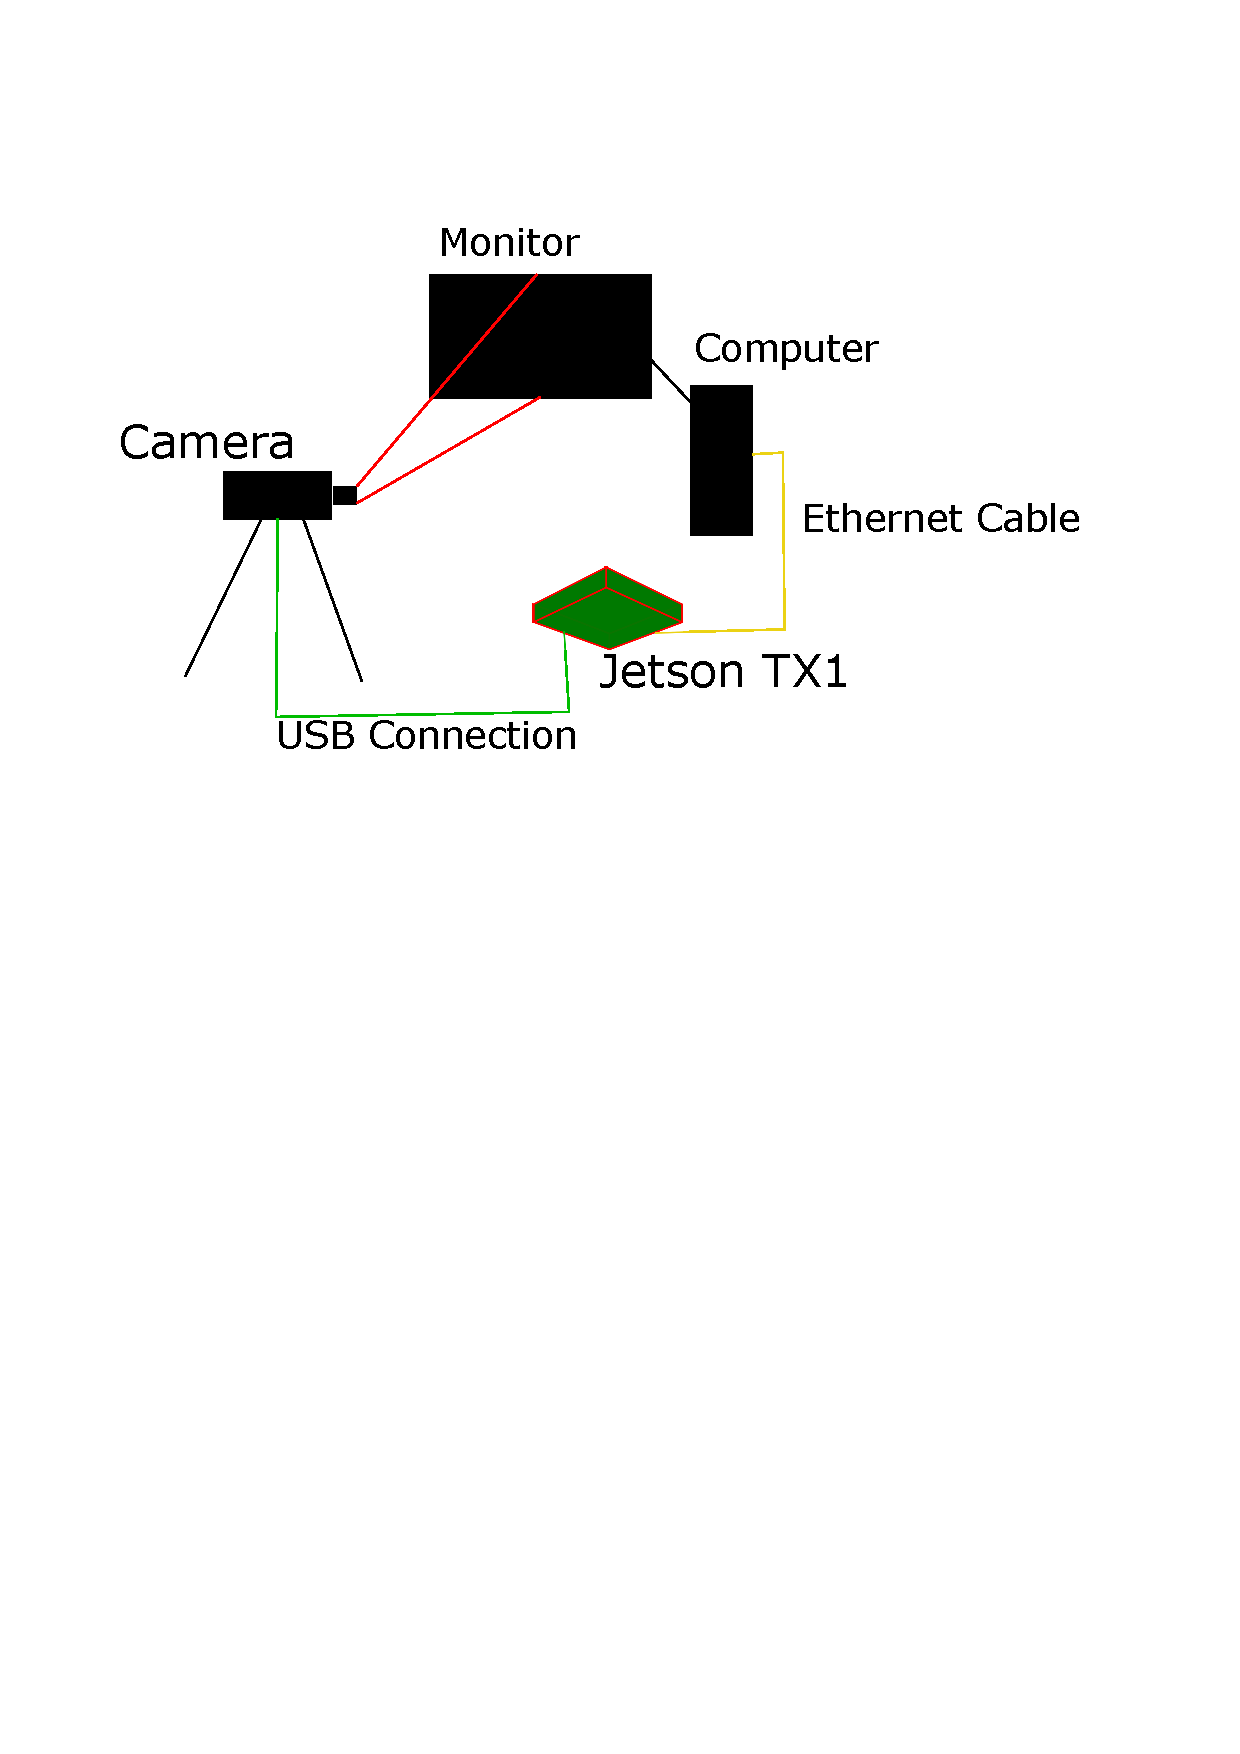
\includegraphics[natwidth=50,natheight=100]{./design.png}
  \caption{Hardware Layout}
  \label{fig:design1}
\end{figure}
Figure \ref{fig:design1} shows the basic layout.

Since the Jetson has to learn how to play the game it needs to be able to see the game.
For this we decided to use the camera sent to us by our client.
This seemed to be the simplest option seeing as we could connect the camera directly to the Jetson.
The camera will be connected to the Jetson and aimed at another screen displaying the game.
The Jetson will first be trained by being given the video input to recognize and characterize objects within the game.
We will set up tables so that the neural net will be able to store information such as the locations of objects.
Once those things are set up it will be able to train itself by playing the game using the controller.
It will base its decisions on the table of information that it stores and eventaully be able to survive the games longer.
Eventually it will learn to respond to certain patterns in the table in order to become better at the game.

\chapter{Conclusion}



\end{document}
